%!TEX root = ./../main.tex
\chapter{Introduction}
% Parte introduttiva dall'A di federica; obbiettivi:
% capire quanto accurata la descrizione Ele CG per ottenere risultati giusti rispetto all'atomistico; complicazione relative all'interazione ele, si sono già affrontati con martini STD cg.
%
% Richiamo a due risultati exp in contraddizione: fig 2 federica con il lavoro di reflettometria a neutroni, Macchirini. Contraddizione -> Simulazioni MD per capire cosa succede meglio
%
% D federica
%
% Stato dell'arte di conti di energia libera di soluti che penetrano in membrana

\begingroup
\introductionStyle

\tocless\section{motivation and objectives}
Metal \acp{NP} play more and more important roles in pharmaceutical and medical technology as diagnostic or therapeutic devices. Metal \acp{NP} can nowadays be engineered in a multitude of shapes, sizes and compositions, and they can be decorated with an almost infinite variety of functionalities. Despite such technological advances, there is still poor understanding of the molecular processes that drive the interactions of metal \acp{NP} with cells. Cell membranes are the first barrier encountered by \acp{NP} entering living organisms. The understanding and control of the interaction of \acp{NP} with biological membranes is therefore of paramount importance to understand the molecular basis of the \acp{NP} biological effects.

This thesis is focused on the study of the interaction between ligand--protected anionic \acp{AuNP} and model biological membranes via computational studies and free energy calculations. Our first aim is to understand how the description of the electrostatic interaction have to be accurate, at \ac{CG} level, in order to obtain quantitative results approaching the atomistic model, in less computational time. A second objective is the estimation of the free energy barriers associated to the transitions involved in the \ac{NP}--membrane interaction using a \ac{CG} \ac{FF} (see chapter~\ref{chap:EmpiricalFF}). Moreover it is important to characterize, at molecular--level, the \ac{NP}--membrane interaction and the structural deformation of the bilayer in presence of the \ac{NP}.%: how does the passive \ac{NP}-membrane interaction happen? What are the physical driving forces leading to the formation of a stable \ac{NP}-membrane complex (electrostatic interactions, hydrophobic interactions...)? How does the composition of the \ac{NP} ligand shell affects such an interaction?

We will now draw the background scenario of the thesis, going more into detail about our motivations and the state of the art of the computational studies in this field.

\tocless\section{relevant experimental results and NP--membrane interaction issues}
Membrane permeation can happen via direct translocation, which is a passive mechanism, or via endocytosis, which on the contrary is an active, receptor--mediated process. Direct translocation is more likely for small ($< 10$~nm) \acp{NP}, while the endocytotic pathway is typical of the larger ones.

Depending on the target application, the \ac{NP} may be required to easily, passively go through the cell membrane, or to bind to specific receptors and enter the cell via a protein--mediated pathway, or even to stably bind to the membrane. The membrane--\ac{NP} interaction results from the complex interplay of electrostatics, hydrophobic interactions, ligand composition, surface ligand organization and, on the membrane side, lipid composition and phase.

In particular it is known form literature that the charge of the surface ligands plays an important role in the toxicity of the functionalized \ac{NP} interacting with lipid membrane. Goodman \etal in \cite{Goodman2004}, via experiment on living cels and bacterial cultures and fluorescence microscopy using multilamellar neutral lipid vesicles, have found that the toxicity mechanism is related to the formation of pores in the membrane that can lead to membrane destruction. Moreover, they found that cationic \acp{AuNP} are more destructive than the anionic one, as we can see from figure~(\ref{fig:goodman}).
\begin{figure}[!ht]
	\centering
	\subfloat[]{%
		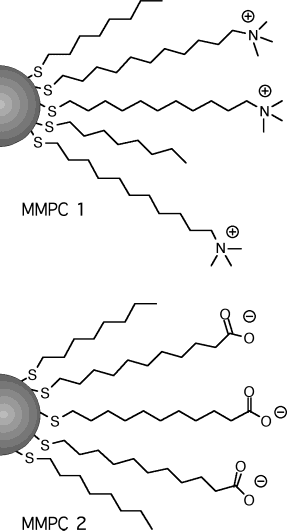
\includegraphics[width=0.2\textwidth]{./img/GoodmanNPs.png}%
	}\qquad\qquad%
	\subfloat[]{%
		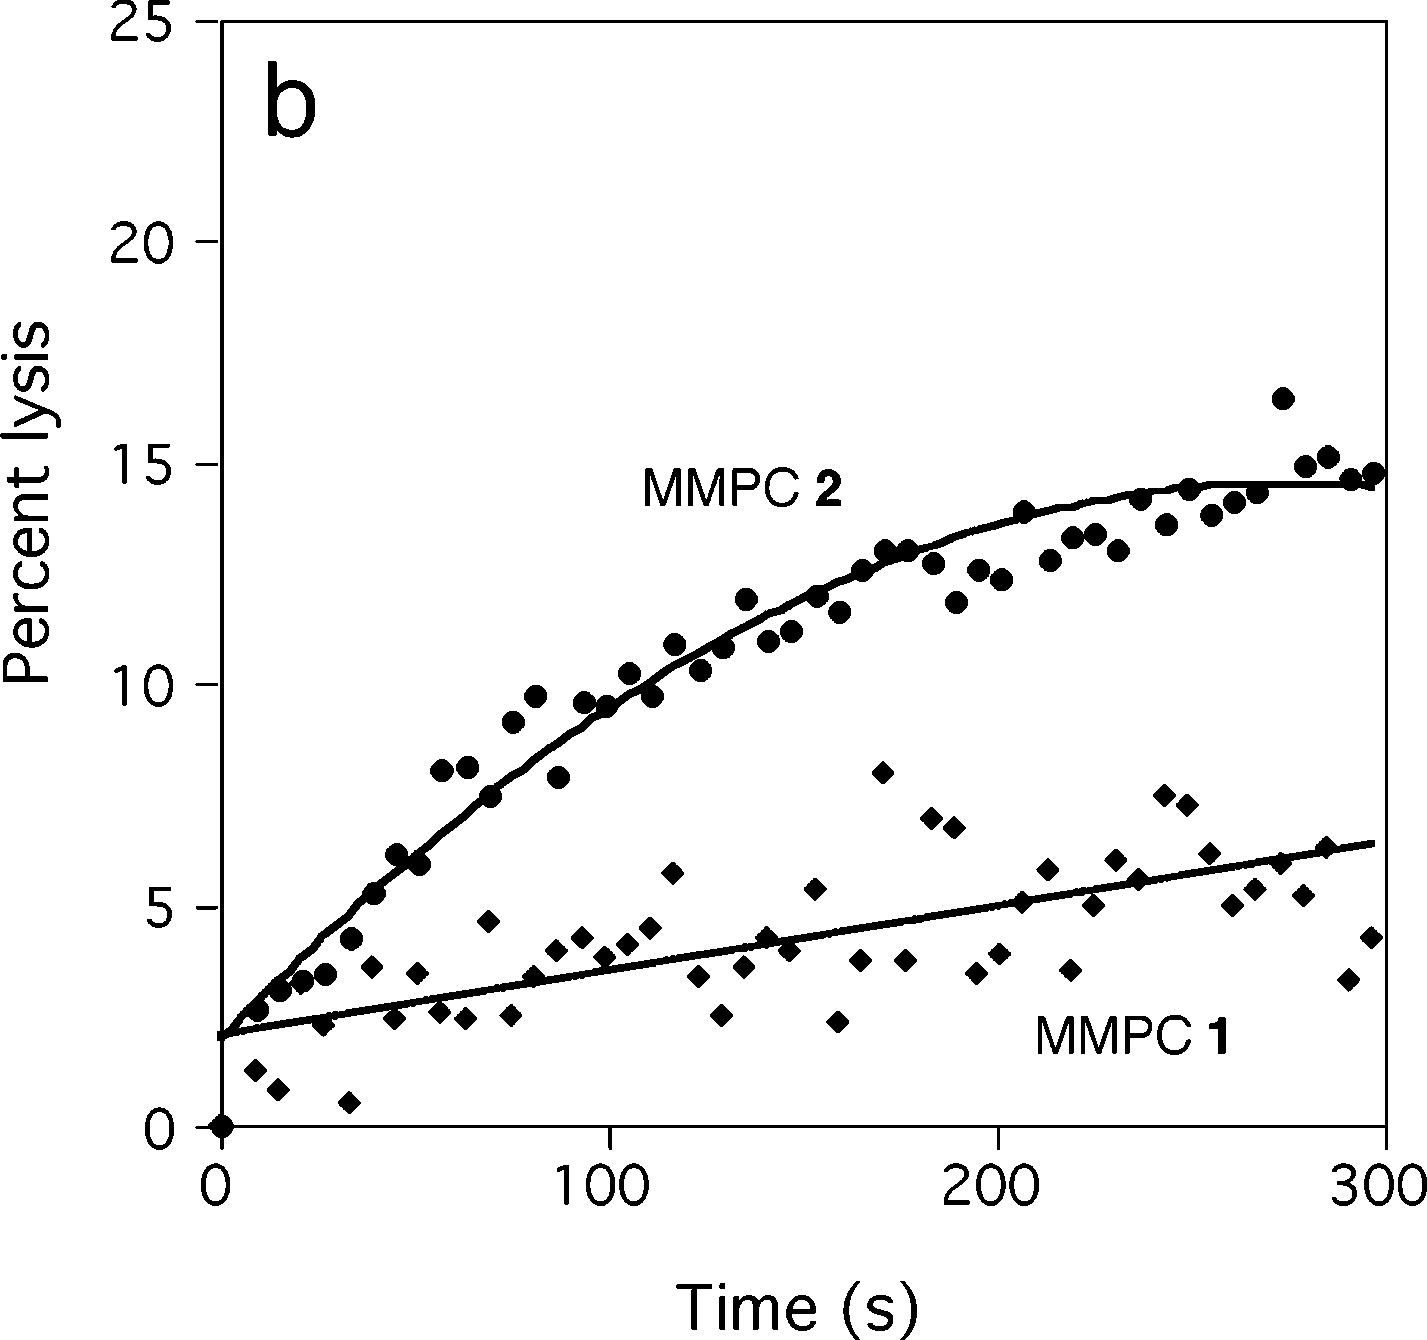
\includegraphics[width=0.4\textwidth]{./img/lysis.png}%
	}%
	\caption{Left: \acp{AuNP} functionalized by a monolayer of neutral and positively charged (MMPC $1$) or negatively charged (MMPC $2$) ligands. Right: Comparison of MMPC $1$ and $2$ in disrupting vesicles made of neutral lipids. In this kind of essays, the disruptive power of the \acp{NP} is quantified by the amount of fluorescent dye that is released from the vesicles. Taken from \cite{Goodman2004}.}%
	\label{fig:goodman}
\end{figure}

More recently, Van Lehn \etal in \cite{VanLehn2013} from experimental results via confocal microscopy images, shown in figure~(\ref{fig:fluorescent}), have demonstrated that anionic \acp{AuNP} can stably blind to the lipid membrane in a non--destructive manner and moreover that they can passively diffuse inside a multilamellar vesicle made of a zwitterionic lipid. The \ac{AuNP} was labelled with the red fluorescent BODIPY dye and solved in a water solution with the multilamellar vesicle and a green fluorescent calcein dye that does not passively diffuse through lipid bilayers.
\begin{figure}[!ht]
	\centering
	\subfloat[calcein fluorescence]{%
		\includegraphics[width=0.28\textwidth]{./img/calcein.png}%
	}\qquad\qquad\qquad%
	\subfloat[BODIPY fluorescence]{%
		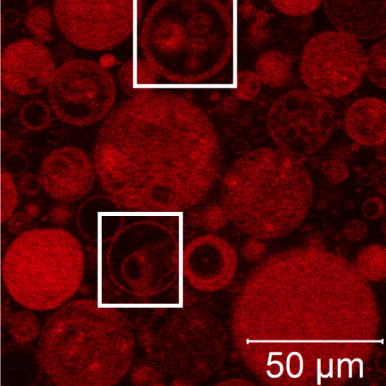
\includegraphics[width=0.28\textwidth]{./img/BODIPY.png}%
	}%
	\caption{Confocal microscopy images of BODIPY--labeled anionic \acp{AuNP} in a solution with multilamellar single--component zwitterionic lipid vesicles and the membrane impermeable dye calcein. Green fluorescence from calcein, left image, was only observed from the vesicle exterior. This means that no vesicles has been destroyed since the calcein can penetrate the vesicle interior only if pores are formed in the lipid membrane. Indicating that anionic \acs{AuNP} do not induce pore formation. BODIPY red fluorescence, right image, was localized to both interior and exterior membranes of the multilamellar vesicles, with a noticeably stronger fluorescence at the interior respect to the background. This suggest a preferential bilayer--\acs{AuNP} interaction and that the \acp{AuNP} can passively diffuse through the lipid membrane in a non--destructive manner. Taken from \cite{VanLehn2013}.}%
	\label{fig:fluorescent}
\end{figure}

In another recent work, Tatur, Maccarini \etal in \cite{Maccarini2013}, made a neutron reflectometry experiment on a floating zwitterionic lipid bilayer supported on a silicon substrate in presence of \acp{AuNP} functionalized with both anionic and cationic ligands. Studying the structural deformation of the bilayer they found that the anionic \acs{NP} are overall more toxic then the cationic one. They found that the latter can passively penetrate into the hydrophobic region of the membrane in a non destructive manner for wide range of temperatures under the liquid--gel transition. Above the liquid--gel transition, instead, they observe that more and more cationic \acp{NP} can permanently penetrate inside the membrane leading to a gradual destabilization of its structure, depending on the quantity of inserted \acp{AuNP}. On the contrary, for what concern the anionic \acp{AuNP}, they observe a drastic change in the structural properties of the bilayer respect to the test sample. The authors suggest that the anionic \acp{NP} do not have the tendency to penetrate inside the lipid membrane. Rather, they interact with its surface strongly dehydrating the floating bilayer. As a consequence the authors suggest a possible decrease in the bilayer thickness and an increase of its susceptibility to disintegrate and to form lipid vesicles. Clearly this results are in contrast with a last two. Thus the importance to perform \ac{MD} simulations to investigate the molecular processes involved in the \ac{NP}--membrane interaction.

Other physico--chemical characteristics of the \ac{NP} ligand shell affect the \ac{NP}--membrane interaction. On top of all, the hydrophobic character of the ligand shell is believed to play a major role. Moreover, what is most intriguing and unexplained is the effect of the ligand composition and surface arrangement on the \ac{NP}--membrane interaction. To date, neither the poration process, nor the binding process, nor the effects of ligands with different degrees of hydrophobicity have been described at molecular level, hindering the design of \acp{NP} with target--specific ligand composition.


\tocless\section{state of the art of the computational studies of aunp--lipid membrane interactions}
Van Lehn \etal \cite{VanLehn2013} have published a computational work concerning the way anionic \acp{NP} penetrate cells membrane. They studied the influence of the size and surface composition of functionalized \acp{AuNP} on the internalization pathway into the cells in addition to the steps through which the process evolves. They used both a thermodynamic--based model and experiments, see figure~(\ref{fig:fluorescent}), to test the hypothesis that the first step in cells penetration is the fusion of the \acp{AuNP} with lipid bilayers, the process being driven by the hydrophobic effect. The hypothesized mechanism relies on the capability of the ligands on the \ac{NP} surface to ``snorkel'' the charged end groups to the aqueous environment thus exposing a greater hydrophobic area to the bilayer core. Van Lehn \etal conclude that the process is size--dependent rather than morphology--dependent and that there exists a critical diameter, dependent on the coating composition, above which fusion with the lipid bilayer becomes unfavorable.

Heikkilä \etal \cite{Heikkila2014} demonstrated, by \ac{MD} simulations, that anionic \acp{AuNP} can adsorb at the surface of neutral lipid membranes. The limited time scale of the simulations performed in their work, which is based on an atomistic \ac{FF} (see chapter~\ref{chap:EmpiricalFF}), did not allow to observe and describe any penetration of the \ac{NP} into the hydrophobic membrane core. To speed--up the process, Van Lehn \etal \cite{VanLehn2014} have considered the interaction between an anionic \ac{AuNP} and a highly curved lipid bilayer, observing the fusion between the \ac{NP} and the membrane.

Gkeka \etal modelled rigid \cite{Gkeka2013} and \ac{CG} \cite{Gkeka2014} (see chapter~\ref{chap:EmpiricalFF}) \acp{NP}, with different arrangements of the charged surface ligands, in the attempt of deriving free energies of transfer from the water phase to the membrane interior for \acp{NP} with different degrees of hydrophobicity.

More recently, in order to speed--up the \ac{MD} simulation and the \ac{NP}--membrane interactions, Federica Simonelli \etal \cite{simonelliThesis} and \cite{ourPaper}, have developed an elastic network for a small \ac{AuNP} and a \ac{CG} model of the functionalizing ligands (see chapter~\ref{chap:membraneNP}). This allowed to two main goals. First to derive the molecular mechanism associated to the interaction between the \ac{NP} and a planar model biological membrane, using a \ac{CG} \ac{FF} and different arrangements of charged surface beads. Second to perform the free energy of transfer of one charged ligands form the entrance leaflet to the opposite one. 


\tocless\section{state of the art of the free energy calculations on lipid membrane solutes translocation}


\tocless\section{contents overview}


\endgroup